\chapter{General discussion} \label{ch:discussion}

\section{ChIP-seq methodology}

With the efforts to optimise the ChIP technique and the development of the NGS technology, ChIP-seq offers a robust and powerful way of studying TF-DNA interactions \textit{in vivo}. It is foreseeable that in future, a ChIP-seq experiment will become cheaper and faster. However, there are also many limitations and biases, both experimentally and bioinformatically, for this method. Therefore, when drawing conclusions based on the ChIP-seq data, one must be aware of the potential problems involved in this technique.

\subsection{Experimental limitations} \label{section:chiplimitation}

The quality of the antibody is the primary limitation of the ChIP-seq experiment. During the immunoprecipitation step, both specific and non-specific proteins will be pulled down, and stringent washes (high concentration of salt) are applied later on. Therefore, an ideal antibody should have high specificity so that less non-specific protein is immunoprecipitated, and high affinity so that stringent washes will not disrupt the antibody-antigen binding. However, such antibodies are not always available. Even if an ideal antibody exists, the epitope recognised by the antibody might be masked or destroyed during the crosslinking step. In our case, we have tested several antibodies for FOXM1 and FOXO3 respectively. The FOXM1 antibody from Santa Cruz Technology (C-20, sc-502) works best in our hands, in terms of specificity, sensitivity and IP efficiency. However, in our hands, none of the tested antibodies for FOXO3 are suitable for the ChIP application (Cell Signalling \#9467, Cell Signalling \#2497, Millipore 07-702, and Abcam ab12162).

When no antibody for ChIP is available, the epitope-tagged version of protein of interest can be used. There are a number of choices for the tags in ChIP-seq experiments: FLAG, Myc, V5, GFP, biotin, all of which have been successfully used in ChIP-seq analyses. We have tested both FLAG (N-terminal) and V5 (C-terminal) tags for FOXO3. V5-tagged FOXO3 cannot be efficiently immunoprecipitated by the antibody after crosslinking (data not shown), while the FLAG tag works well for the ChIP of FOXO3. Therefore, a FLAG- tagged FOXO3 stable cell line was generated and used for the ChIP-seq study of FOXO3. When the epitope-tagged version of a protein is used for ChIP-seq, it is generally preferred to have the expression level of the exogenous protein comparable to the endogenous one, \textit{i.e.} not to overexpress, because the overexpression might artificially cause the protein to bind many other places than the endogenous protein. However, this assumption has never been rigorously tested. According to a very recent study which investigated the genome-wide binding events of Olig2 in mouse embryonic stem cells, the binding profiles (number of binding sites, locations of binding sites \textit{etc.}) between the endogenous Olig2 and overexpressed (more than 5 fold) V5-tagged Olig2 are very similar (\cite{mazzoni2011embryonic}). Therefore, whether overexpression can cause artificial binding events still needs to be thoroughly investigated.

Another potential problem of ChIP-seq is regional bias. Usually, during the library preparation step, only small fragments that are within the optimal size range for the NGS application are selected (100 - 200 bp for SOLiD, 300 - 500 bp for Illumina). However, many regions in the genome, like heterochromatin, are highly compacted and therefore are difficult to sonicate. Therefore, those regions that are refractory to sonication tend to be under-represented in ChIP-seq analyses (\cite{teytelman2009impact}). In contrast, regions within open chromatin are generally easier to shear, which often yields higher coverage during the sequencing (\cite{auerbach2009mapping}). Hence, the chromatin state will bias the downstream data analysis.

GC-bias is another issue of ChIP-seq experiments. Since GC-rich sequences are difficult to amplify by the PCR reaction, some high GC-content sequences might be lost during early library preparation steps (\cite{aird2011analyzing}). However, for some unknown reasons, GC-rich sequences tend to be over-represented during the sequencing step on the Illumina platform, which will influence the downstream peak finding steps (\cite{dohm2008substantial,cheung2011systematic}). On the other hand, the SOLiD platform seems to have difficulty recovering GC-rich sequence during the run (see more details in the \textbf{Appendix}). Therefore, when analysing factors, like zinc finger proteins which bind to GC-rich sequences, the data should be treated with caution. Recently, some methods, both experimental and bioinformatical, have been developed for the Illumina platform to reduce these biases (\cite{aird2011analyzing,cheung2011systematic}), and these methods might be useful in future applications.

In addition, sequencing depth is also an important factor when doing ChIP-seq experiments. Intuitively, one criterion to determine whether sufficient sequencing depth has been reached is that no further binding sites can be detected with additional reads (\enquote{saturation point}). However, different transcription factors and peak calling algorithms have various saturation profiles (reviewed in \cite{park2009chip-seq:}). With the advancement of sequencing technology, recent ChIP-seq data sets often contain 10 - 30 M reads per factor in the human genome. Lately, a study suggests such a level of sequencing depth might not be enough for some transcription factors and histone marks (\cite{chen2012systematic}). However, this
suggestion is based on experiments performed in \textit{Drosophila} S2 cells (\cite{chen2012systematic}). Our FOXM1 ChIP-seq experiments yielded 27,892,797 and 8,906,067 uniquely mapped reads for the first and second replicate respectively, and more than 99\% of the reads are not in the FOXM1 binding peaks, indicating that the majority of the mapped reads are actually background, which is a common phenomenon in ChIP-seq analyses (reviewed in \cite{pepke2009computation}). Although it has lower sequencing depth, the second replicate has recovered most FOXM1 binding sites and exhibits relatively higher signals than the first replicate (\textbf{Figure \ref{fig:fig12}}). Therefore, at least in the FOXM1 case, it seems that the current standard sequencing depth (10 - 30 million reads) is enough.

\subsection{Bioinformatical limitations}

After the sequencing, intensive bioinformatic analyses need to be done to extract biological meaning (enriched regions in the case of ChIP-seq) from the huge amount of short sequencing tags.

The first daunting task is mapping the short sequencing reads to reference genomes. Since the sequence of the human genome is not random, highly repeated and degenerated regions are difficult to map. Many computational algorithms are available for mapping, including the most commonly-used ones: MAQ (\url{http://maq.sourceforge.net/}), BOWTIE (h\url{ttp://bowtie-bio.sourceforge.net/index.shtml}), and BFAST (\url{http://bfast.sourceforge.net/}), as well as programs provided by the sequencing companies: ELAND (Illumina) and Corona-Lite (SOLiD). During the reads alignment, a certain extent of mismatch (usually up to 2 mismatches) should be allowed due to sequencing errors, SNPs, and indels or differences between the interrogated genome and the reference genome (reviewed in \cite{park2009chip-seq:}). One of the main issues of mapping is the way of dealing with reads that can be aligned to multiple regions of the genome. Usually, those reads are discarded, and only reads that are uniquely mapped to the genome are preserved. The mapping algorithms also provide the options to retain the reads that can be mapped to multiple positions of genome, given that one position is mapped better than the others. Whether to only keep uniquely mapped reads or not will slightly affect the downstream identification of binding events. We have tried both methods in our FOXM1 and FOXO3 ChIP-seq data sets, and found out that the overall binding patterns and conclusions are not affected (data not shown).

Another bioinformatically challenging task for ChIP-seq is the peak calling. After the alignment of reads, one needs to identify statistically significant enriched regions, \textit{i.e.} binding events. Dozens of peak calling algorithms are available. In general, there are two major types of peak calling methods: sliding window based method (\textit{e.g.} MACS) and kernel density estimation based method (\textit{e.g.} QuEST). The former divides the genome into small overlapping or non-overlapping windows and calculates the number of reads and statistical significance within each window based on certain probability models (\textit{e.g.} Poisson and binomial distributions); the latter is a non-parametric (\textit{i.e.} does not rely on any distributions) method to facilitate finding the aggregation of densely packed short sequencing reads which leads to the identification of binding events. Direct comparisons of many peak callers were performed recently (\cite{wilbanks2010evaluation,feng2011peakranger:}). Although certain peak callers seem to outperform others, due to poorly defined standards in some cases, no conclusive remarks can be drawn from the comparisons (\cite{wilbanks2010evaluation}). In our study, MACS and HOMER are used for the peak calling, because: 1) MACS is widely used and has been shown to be good at detecting both punctate and broad peaks; 2) HOMER is a multi-functional software suite which is user- friendly and easy for wet lab biologists to use, and it also has been demonstrated to be robust for analysing both transcription factor and histone modification ChIP-seq data (\cite{heinz2010simple,lin2010a,wang2011reprogramming}).

Despite the lack of benchmarks for the data analysis, high confidence binding events are always revealed no matter what method is used. Some specific binding/regulatory events at certain loci will be affected by the computational methods used. For example, in our FOXK2 and FOXO3 ChIP-seq data, MACS and HOMER revealed similar numbers of binding events respectively, but only 50 \textasciitilde 60\% of the binding sites were called by both algorithms. However, the overall conclusions from a ChIP-seq experiment will not be affected by the method used. This can be demonstrated by the fact that most ChIP-seq results conducted in different labs and using different methods are still very consistent with known biological functions and biochemical properties of the factor of interest. Therefore, by performing biological replicates or using various analytical tools, the data extracted from ChIP-seq experiments can be very robust (\cite{wilbanks2010evaluation}).

\section{Genome-wide TF-DNA binding events}

The interaction between DNA and transcription factors is the fundamental basis for generating transcriptional networks. The specific structures and amino acids within the DNA-binding domains mean that transcription factors can only bind to certain DNA sequences. However, the \textit{in vivo} DNA-binding events of transcription factors are determined by more than the simple protein-DNA recognition.

\subsection{Only a small proportion of consensus binding sites are occupied by a factor}

The first complicated scenario is that not all potential binding sites are actually occupied by a transcription factor. Given a certain cell type at a certain condition, a transcription factor seems to only select a subset of available consensus sequences to bind. The GTAAACA sequence occurs 472,221 times in the human genome according to the unmasked hg18 assembly. In terms of sequence, there should be 472,221 available binding sites for any given Forkhead transcription factor. Considering the degenerate nature of TF-DNA binding, this number is still an underestimation. However, only 1.6\% and 0.34\% of the GTAAACA sequences are occupied by FOXK2 and FOXO3 respectively. Similar observations are also seen for many other transcription factors (reviewed in \cite{pan2010mechanisms}). It seems this is a general phenomenon related to the \textit{in vivo} DNA-binding events of transcription factors.

It has been suggested that nucleosomes are the barriers that block a transcription factor binding to its consensus sequence (reviewed in \cite{li2007the}). Therefore, one reason that the majority of consensus sequences are not bound by the transcription factors could be that they are compacted within nucleosomes. However, some proteins like Forkhead transcription factors can act like pioneer factors which are able to bind to condensed chromatin (reviewed in \cite{zaret2011pioneer}). Hence, the nucleosome occupancy only partially explains why a consensus site is not bound by a factor. In addition, DNA methylation within the consensus sequences may also contribute to the DNA binding of a transcription factor. For example, the methylation of the CpG within the CTCF consensus motif blocks its binding (\cite{bell2000methylation}), while ZBTB33 (also known as Kaiso) only binds to methylated GC-rich sequences (\cite{yoon2003n-cor}). However, there are no CpGs within the Forkhead consensus, and this is not likely to be relevant here.

Another mechanism that controls transcription factor selectivity is the cooperative binding with other proteins. Since transcription factors are thought to never work alone, they always bind to \textit{cis}-regulatory modules which are often occupied by a number of transcription factors at the same time (reviewed in \cite{farnham2009insights}). Therefore, the binding of a transcription factor is often affected by the binding of other transcription factors. Indeed, when comparing the genome-wide binding events of FOXM1, FOXO3 and FOXK2 to the ChIP-seq of many other transcription factors from the ENCODE project, the binding sites of FOXM1, FOXO3 and FOXK2 are usually associated with other transcription factor DNA-binding events, although there are no apparent connections among them (\textbf{Figure \ref{fig:fig52}}, note the overlap between grey bars and coloured bars). In general, a transcription factor is more likely to bind to the regions where there are other transcription factor binding events nearby.

\begin{figure}[!h]
    \centering
    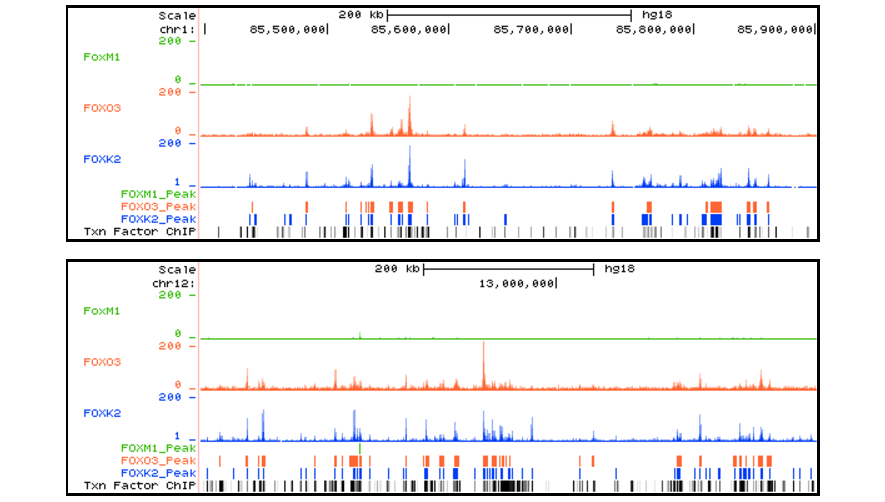
\includegraphics[width=0.9\textwidth]{chapter4/figures/fig52.pdf}
    \caption[Examples of the overlapping of binding events for FOXM1, FOXO3, FOXK2 and other transcription factors from the ENCODE project]{\textbf{Examples of the overlapping of binding events for FOXM1, FOXO3, FOXK2 and other transcription factors from the ENCODE project.} Genomic binding profiles of FOXM1, FOXO3 and FOXK2 from a region of chromosome 1 or chromosome 12. The binding events of FOXM1 (red), FOXO3 (orange) and FOXK2 (blue) are shown as coloured bars below their binding profiles. The binding sites of all other available transcription factors are shown in grey bars at the bottom. This data is taken from the ENCODE project which contains more than 20 transcription factor ChIP-seq data sets in 25 different cell types. The intensity of the grey bar indicates the number of transcription factors bound in that region. Note the overlap between coloured bars and grey bars.}
    \label{fig:fig52}
\end{figure}

\subsection{Not all binding events involve the consensus motifs}

Another common phenomenon in the transcription factor ChIP-seq data is that not all binding events contain the consensus motif of the protein of interest. In the FOXK2 and FOXO3 binding regions, only \textasciitilde 25\% of them contain the strong motif GTAAACA. When taking the weaker motif (RTMAAYA) into account, there are still \textasciitilde 40\% binding events that do not contain a consensus motif. Since formaldehyde can crosslink both protein-DNA and protein-protein interaction during the ChIP experiments, a protein can be indirectly linked to the DNA by interacting with other DNA-binding factors. In fact, in the FOXK2 and FOXO3 cistromes, motifs bound by other transcription factors (\textit{e.g.} AP1, CTCF and ETS1) occur more frequently within the peaks which do not contain the RTMAAYA motif (data not shown). Therefore, the differential enrichment of different motifs and the overlapping with various transcription factors within FOXK2 and FOXO3 binding regions suggest that some indirect DNA contact exist in these two factors. This indirect recruitment is a universal mechanism used by many other transcription factors to bind to chromatin \textit{in vivo} (reviewed in \cite{farnham2009insights}).

FOXM1 seems to be an extreme example where its consensus motif is not enriched within its binding regions at all. A previous study indicates that FOXM1 has very low affinity ($\mu$M) to the Forkhead consensus sequence, presumably due to the lack of sugar-phosphate backbone contacts with the DNA (\cite{littler2010structure}). In the crystal structure of the DNA-binding domains of Forkhead transcription factors, the third $\alpha$-helix ($\alpha$3) reaches into the major groove of the DNA, making sequence-specific contacts with the DNA via hydrogen bonds and van-der-Waals interactions (\textbf{Figure \ref{fig:fig53}}, yellow arrows). In other Forkhead transcription factors like FOXA, FOXK, and FOXO, the second \enquote{wing} (W2) which consists of positively charged amino acids also interacts with the DNA at the sugar- phosphate backbone, the minor groove and the major groove (\textbf{Figure \ref{fig:fig53}}, white arrows). In stark contrast, the W2 of FOXM1 adopts a unique structure which diverges away from the DNA (\textbf{Figure \ref{fig:fig53}}, the rightmost panel, the white arrow). The lack of W2-DNA interaction might be the reason that FOXM1 possesses such a low affinity to the Forkhead consensus (\cite{littler2010structure}). Interestingly, a recent study has solved the crystal structure of ASH2L and revealed that it also holds a Forkhead-like winged-helix domain. The affinity of ASH2L to its consensus sequence is also very low ($\mu$M), presumably due to its negatively charged W2 which cannot stably interact with the DNA (\cite{sarvan2011crystal}).

\begin{figure}[!h]
    \centering
    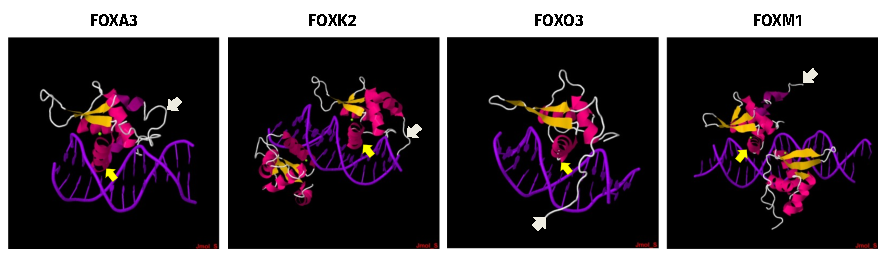
\includegraphics[width=\textwidth]{chapter4/figures/fig53.pdf}
    \caption[Comparisons of crystal structures of the DNA-binding domains of FOXA3, FOXK2, FOXO3 and FOXM1 in a complex with Forkhead consensus DNA sequence]{\textbf{Comparisons of crystal structures of the DNA-binding domains of FOXA3, FOXK2, FOXO3 and FOXM1 in a complex with Forkhead consensus DNA sequence.} Pictures are taken from the Protein Data Bank. The $\alpha$3 and the W2 of each DNA-binding domain are indicated by the yellow and white arrows respectively.}
    \label{fig:fig53}
\end{figure}

It is possible that such a low affinity to DNA might yield the small number of binding sites for FOXM1. Considering there are multiple Forkhead proteins present within the cell, it is reasonable to speculate that FOXM1 is unable to compete with other Forkhead proteins, such as FOXK2 and FOXO3, to bind the canonical Forkhead consensus. Therefore, the Forkhead consensus is not enriched in the FOXM1 cistrome. This is, indeed, supported by our ChIP-seq studies.

\section{Genome-wide DNA-binding events among family members}

Since members within the same family can bind to the same consensus sequence, and often multiple members from the same family are expressed in a cell, the binding events among family members can be very complicated.

First, the number of binding sites varies greatly within individual members. The difference of the number of binding sites among Forkhead proteins is a good example (\textbf{Table \ref{table:fkhtfschip}}). The Forkhead DNA-binding domain has been shown to structurally resemble linker histone (\cite{clark1993co-crystal}), indicating that the Forkhead transcription factors can stably interact with DNA. Consistent with this notion, certain Forkhead transcription factors, like FOXA1 and FOXI1, have been proven to be able to bind condensed chromatin (\cite{cirillo1998binding,yan2006the}). Therefore, one often expects Forkhead transcription factors have many binding sites. Indeed, many Forkhead transcription factors, like FOXA1, FOXP3 together with our FOXK2 and FOXO3, do meet that expectation. However, some Forkhead transcription factors, like FOXP2 and FOXM1, have relatively fewer binding sites than others (\textbf{Table \ref{table:fkhtfschip}}). This difference can be partially derived from the endogenous protein levels, the cellular conditions, the cell lines and the antibodies used in the experiments. In addition, the small number of binding sites of FOXM1 and its extreme low affinity to the DNA imply that protein-DNA affinity might also contribute to the number of binding sites in vivo, and our FOXM1 ChIP-seq studies support this idea.

Second, family members often have both redundant and specific binding events despite the fact that they all bind to the same sequence \textit{in vitro}. It has been suggested that nucleotides within and flanking the core sequence can influence the binding of individual members. In this study, although no discernible preferences can be detected within the Forkhead consensus between FOXK2 and FOXO3, the nucleotides flanking the core consensus contribute to the DNA binding of FOXK2 both \textit{in vivo} and \textit{in vitro}. Similar observations are also seen within members from the ETS-domain transcription factor family (\cite{wei2010genome-wide}). In addition, a recent PBM study suggests that besides the consensus motif (primary site) recognised by a transcription factor, most proteins can also bind to multiple distinct DNA motifs (secondary, tertiary sites \textit{etc.}) (\cite{badis2009diversity}). In some cases, the binding of a transcription factor to the secondary site is equally efficient as to the primary site (\cite{badis2009diversity}). Many transcription factors from the same family have very similar primary site, but the differences among their secondary sites can be quite different (\cite{badis2009diversity}). For example, among all five tested mouse Forkhead transcription factors, the primary sites for them are Forkhead-like consensus containing GTAAACA, but the secondary sites are relatively more variable: TAACA for Foxa2, AYAACA for Foxj1 and Foxk1, CAHAACA for Foxj3 (\textbf{Figure \ref{fig:fig54}}). Therefore, it is tempting to speculate that the differences of the secondary sites of FOXK2 and FOXO3 might also contribute to their \textit{in vivo} DNA binding. Unfortunately, such data is not available yet.

\begin{figure}[!h]
    \centering
    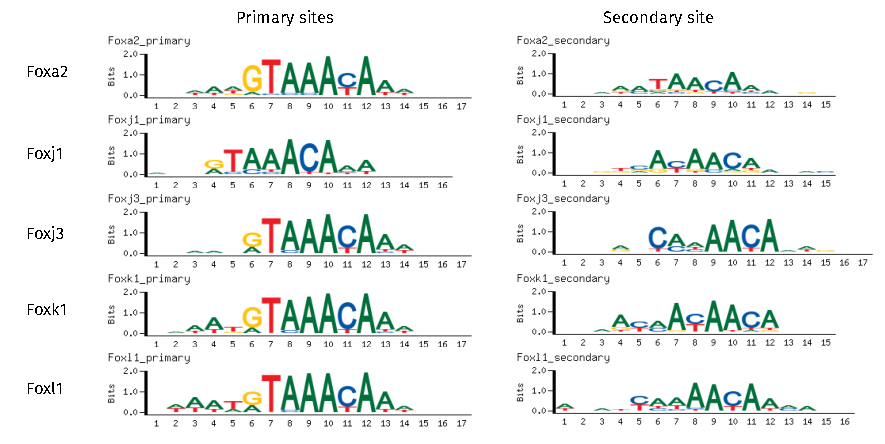
\includegraphics[width=0.9\textwidth]{chapter4/figures/fig54.pdf}
    \caption[Comparison of the primary and the secondary binding sites of five mouse Forkhead transcription factors]{\textbf{Comparison of the primary and the secondary binding sites of five mouse Forkhead transcription factors.} The PBM data of five indicated mouse Forkhead transcription factors are from the Uniprobe database (\cite{Newburger2009-uc}).}
    \label{fig:fig54}
\end{figure}

Another conundrum is the binding relationship of family members within their redundant binding events. When only one site is available within the redundant binding region, the binding of family members to the binding site is generally thought to be mutually exclusive. Therefore, one often expects competition between family members on the same site, unless they can form a complex. Indeed, competition of the binding between family members has been observed \textit{in vitro}, in yeast and in human (\cite{pierce2003sum1,boros2009overlapping,zhou2011integrated,lickwar2012genome-wide}). However, in this study, we failed to identify any relationship between the binding of FOXK2 and FOXO3 at their shared peaks, since changes in FOXK2 ChIP signals do not affect the FOXO3 ChIP signals and vice versa. The relationship of binding among family members on the same site might be more than just simple competition. Indeed, a recent study using a modified ER (ER pBox) which possesses the same binding specificity as GR demonstrates that these two proteins fail to exhibit any competition even though they are thought to bind exactly the same site (\cite{voss2011dynamic}). Therefore, similar to the ER pBox and GR, one possible explanation for this is that the binding between FOXK2 and FOXO3 to the DNA is quite dynamic, that is, the residence time for the proteins at the DNA is very short. In this case, the available binding site is never really saturated, leading to a consequence that multiple family members can bind to the exact the same site without competing with one another. This is in contrast to a long-residence time binding situation where the available binding site is occupied by one family member for a relatively long time (saturated), and this binding can be competed by other family members when the concentrations of proteins are changed (\textbf{Figure \ref{fig:fig55}}).

\begin{figure}[!h]
    \centering
    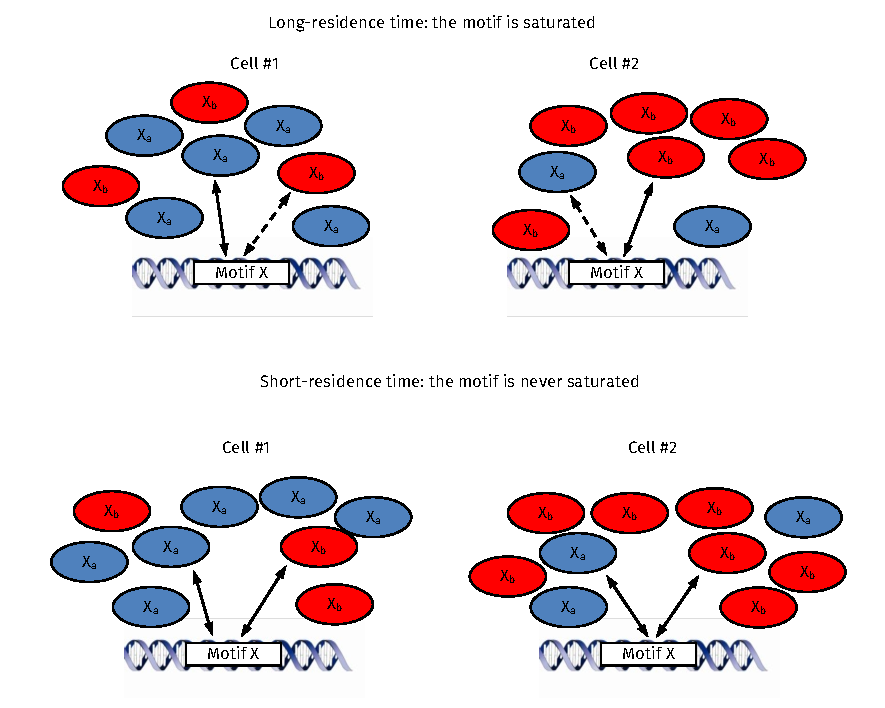
\includegraphics[width=0.9\textwidth]{chapter4/figures/fig55.pdf}
    \caption[Two possible models of TF-DNA occupancy \textit{in vivo}]{\textbf{Two possible models of TF-DNA occupancy \textit{in vivo}. Top,} long-residence time binding. Members within the transcription factor family \textbf{$X$} can bind to their consensus Motif \textbf{$X$}. Long-residence time binding (black lines) of a family member (\textbf{$X_a$} or \textbf{$X_b$}) makes the Motif \textbf{$X$} saturated which is less accessible (dotted lines) to other family members (\textbf{$X_a$} or \textbf{$X_b$}). \textbf{Bottom,} short-residence time binding. Members bind to the Motif \textbf{$X$} in a \enquote{hit-and-run} manner, and the Motif \textbf{$X$} is always available for the binding regardless of the concentrations of family members.}
    \label{fig:fig55}
\end{figure}